% Appendix Template

\chapter{A Fringe-Tracker for BETTII} % Main appendix title

\label{AppendixB} % Change X to a consecutive letter; for referencing this appendix elsewhere, use \ref{AppendixX}

\section*{Abstract}
We present the design of a fringe tracking system for the Balloon Experimental Twin Telescope for Infrared Interferometry (BETTII). BETTII is a balloon-borne, far-infrared, 8~m-baseline interferometer with two 50~cm siderostats. Beams from the two arms are combined in the pupil plane to enable double-Fourier, spatio-spectral interferometry. To maintain the phase stability of the system, we need to actively correct of the optical path difference (OPD) between the two arms. The fringe-tracking system will work in the near-infrared and will use a reference star within the field of view to achieve two goals: overlap the beams coming from the two siderostats, and track the location of the central fringe packet, which is a measure of the OPD. The fringe tracker will share most of the optical train with the science instrument. This system is part of the overall control architecture that feeds fast steering tip/tilt mirrors and a warm delay line to ensure proper beam combination and OPD control for the science instrument. This paper investigates the different sources of perturbations that are expected at float altitude, and derives the sensitivity of the fringe-tracking system. We show progress on validating our design using a visible light, broadband Mach-Zehnder interferometer that was developed at NASA/GSFC. This system demonstrates the viability of our OPD determination approach and provides a means of testing and characterizing several OPD determination and control algorithms.  


\section{Introduction} \label{sec:INTRO}
BETTII is a balloon-borne payload aimed at pioneering a new generation of free-flying interferometers. The science instrument is based on the concept of spatio-spectral interferometry \citep{Mariotti:1988vea}, which can be summarized in three steps: 1) interfere the beams from two light collectors separated by a distance $B$; 2) scan the delay between those two beams to create interferograms and obtain the spectrum of each source in the field through Fourier transform spectrometry; 3) repeat the process for several orientations and baselines to fill the UV-plane. The Wide-field Imaging Interferometer Testbed \citep{Rinehart:2010hq} (WIIT) is a laboratory testbed at NASA/GSFC which has demonstrated the viability of this method in reconstructing complex spatio-spectral scenes \citep{Lyon:2008cna}. This method is planned to be used in space on future missions like SPIRIT \citep{Leisawitz:2007if} and SPECS \citep{Harwit:2006hl}.


BETTII implements this method over a 2'$\times$2' field of view (FOV) in two simultaneous science bands: 30-50~$\um$ (the short band), and 60-90~$\um$ (the long band). These bands are inaccessible from the ground due to absorption and emission from the atmosphere. At 35~km altitude, above 99.6\% of the atmosphere, one can do science in these bands. With a fixed baseline size $B=8$~m, BETTII will provide an angular resolution $\lambda/B\sim 1$" and $\sim 2$" in the short and long band, respectively. The main science goal of BETTII's first flight is the study of star formation in the centers of nearby clusters, where the protostars are very bright at our wavelengths and have typical angular separations on the order of arcseconds. 

It is critical to observe these star-forming regions at very high angular resolution in order to understand the physical processes driving the star formation and to discriminate between the various theories currently explaining clustered star formation. BETTII will help answer these questions by simultaneously resolving individual emission regions separated only by $\sim 1$", and by providing low resolution ($R\sim 35$) spectra of these regions.

BETTII consists of an 8~m carbon fiber structure with two flat mirrors (the siderostats) with a 50~cm diameter collecting area on the sky. They redirect light towards the telescopes, composed of a primary and a secondary mirror, located on each side of a central dewar (see Fig. \ref{fig:Structure}). The afocal telescope achieves a 20:1 compression ratio. The dewar is composed of an external liquid nitrogen volume at 77~K, and an internal liquid helium volume at 4~K, in order to provide the appropriate environment for the far-infrared science detectors. %The mechanism that scans the delay between the two beams to produce science interferograms is located inside the 4~K volume, hence is referred to as the Cold Delay Line (CDL).

Spatio-spectral interferometry requires precise knowledge of the optical path difference (OPD) between the incoming beams for two reasons. First, as we scan the delay line and measure the intensity modulation (or fringes) on the science detectors, it is important to be able to match a given intensity measurement with a given OPD, in order to convert the interferogram to a spectrum, and to coherently add multiple interferograms together to build up the signal-to-noise ratio. Second, as we look at the same scene under different orientations, one needs to be able to reference all interferograms to the same phase reference in order to properly reconstruct the scene.

\begin{figure}[ht!]
\begin{center}
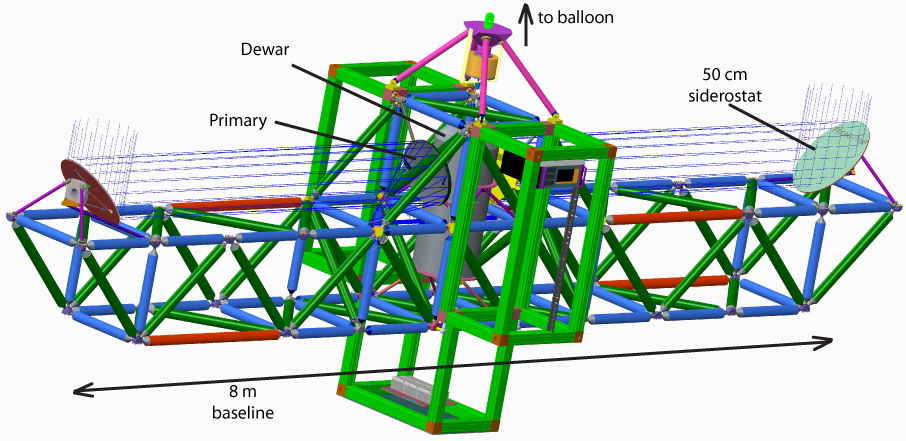
\includegraphics[width=1\textwidth]{Figures/BETTII_Top_Level1.png}
%{Two snapshots of BETTII's carbon fiber gondola and external optics. To the left, one early design is shown, without most of the holding structures for the optics. To the right, a more recent model is shown, with additional elements to connect the optics and to connect to the balloon train. This structure has exceptional thermal properties, and very high frequency vibration modes.}
\caption{BETTII's gondola.}%The 25 mm collimated beam then is sent to a delay line (in one arm) and to a K-mirror (on the right). The K-mirror rotates along with the siderostats to produce proper field rotation. The collimated beam is then sent into a 77 K cold volume of the cryostat, where it is split between the science channel and the fringe tracking unit. The science instrument is in a 4K volume. The science detectors operate at 450 mK. Within the dewar, a cold delay line (CDL) constantly scans the OPD, while the warm delay line (WDL) outside the dewar tries to keep ZPD within the appropriate range for the CDL to cover our total field of view.}
\label{fig:Structure}
\end{center}
\end{figure}

One solution for obtaining this path knowledge is to monitor the OPD using interferometric fringes on a reference star within the field of view. On BETTII, this will be achieved with a near-infrared (NIR) interferometer, part of the Fringe Tracking Unit (FTU). The FTU will combine the two beams of the interferometer to achieve NIR fringe tracking using real-time OPD measurement and compensation. The
BETTII implementation has a warm delay line (WDL) to compensate for path changes in the optical train outside the dewar, and a cold delay line (CDL) inside the dewar to create the path delay scanning required for the spatio-spectral imaging.

The science case is discussed elsewhere\cite{Rinehart:2010p2318}. The details of the payload design are discussed in Rinehart et al., 2012 (these proceedings). Benford et al., 2012 (these proceedings) discuss the environment at float in some detail. This paper will focus on the FTU, and is organized as follows. In section \ref{sec:FTU}, we describe the FTU's role, concept and design. In section \ref{sec:PARAMS}, we detail its parameters and derive the sensitivity of the tracking system. In section~\ref{sec:TESTBED}, we show results from a prototype testbed developed at NASA/GSFC to implement several fringe tracking algorithms for BETTII.

\section{THE FRINGE TRACKING UNIT}\label{sec:FTU}

\subsection{Enabling BETTII science}
\subsubsection{Requirements derived from the science}
\label{subsubsec:Reqs}

Two main requirements derive from the science. First, in order to minimize fringe visibility loss, the two incoming beams need to stay overlapped to better than $\sim$~1.5". Second, in order to interpret the science interferograms, the OPD needs to be known to within $\sim 2~\um$, 1/20 of the shortest science wavelength. It is also important to maintain the location of Zero Path Difference (ZPD) close to the center of the CDL, in order to always be scanning the whole field of view at the science wavelengths.

\subsubsection{Expected perturbations}
The relative optical path lengths along the two arms are sensitive to motions of the gondola, telescope pointing errors, and motions generated within BETTII itself. Several other balloon missions \citep{Fixsen:1996kha} have identified multiple pendulum modes of the payload, which are to be expected at float. They have characteristic periods from 2 to 30 seconds and amplitudes of up to $\sim 10$' relative to the gravity vector. Despite the large amplitudes of these modes, these same balloon missions have shown the ability to robustly stay pointed at the target to within an arcminute, because these motions are very regular and smooth.

Pointing errors will impact the OPD because the baseline vector (the vector connecting the centers of the two siderostats) is not always in the plane perpendicular to the line of sight to the science source. With a baseline $B=8$~m, if the baseline vector is tilted by 1' with respect to this plane, it creates a $2.4$~mm OPD perturbation, which is a very large value compared to our science wavelength. A tilt of 1" creates a 40~$\um$ OPD error.

However, these pointing errors can be measured in real time, and the OPD they generate can be compensated by the WDL in order to meet the science requirements. This advantage allows BETTII to provide arcsecond level resolution without requiring arcsecond level pointing stability of the gondola.

Other perturbations also come into play, such as the ones caused by thermal gradients, the momentum wheels, the actuators themselves. These perturbations are being minimized through careful engineering design and by maximizing the symmetry of the two optical arms of BETTII; this takes advantage of the fact that interferometry is only sensitive to the relative path difference, not the absolute path. To the best of our knowledge, \textit{all high frequency ($\gg  1$~Hz) perturbations will be excited by the payload itself}. In principle all these perturbations can be measured during testing on the ground.


\subsection{Description of the fringe tracking unit}\label{subsec:DESCRIPTION}

The FTU has two components: an Angle Tracker (AT), which overlaps the two beams with high accuracy; and a Fringe Tracker (FT), which measures and corrects for the net OPD up to a dichroic located inside the dewar. That dichroic splits the NIR light from the science bands. 
\begin{figure}[ht!]
\begin{center}
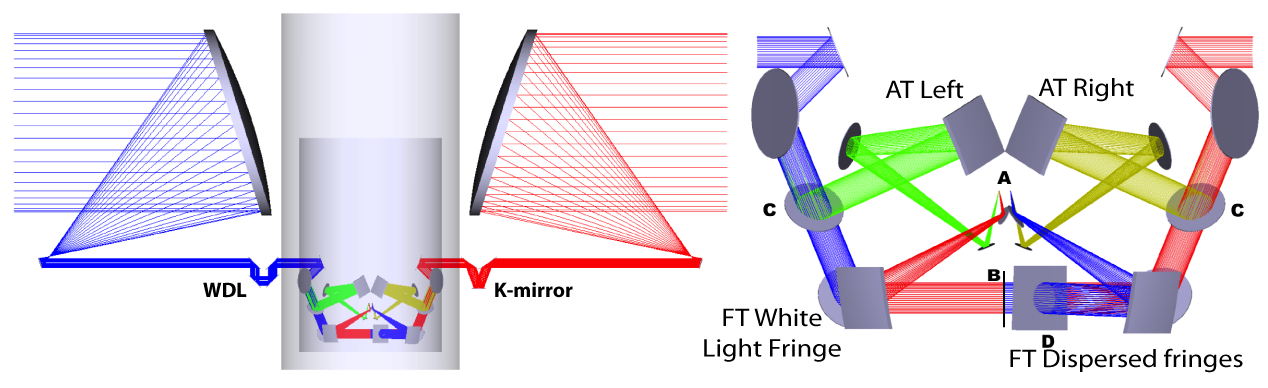
\includegraphics[width=1\textwidth]{Figures/Dewar_FT2.png}
%{Two snapshots of BETTII's carbon fiber gondola and external optics. To the left, one early design is shown, without most of the holding structures for the optics. To the right, a more recent model is shown, with additional elements to connect the optics and to connect to the balloon train. This structure has exceptional thermal properties, and very high frequency vibration modes.}
\caption{The Fringe Tracking Unit on BETTII. Left: Optical path from the primaries to the FTU detectors. In the dewar, represented by the gray rectangle, only the FTU optics are shown. The optics for the science instrument go above. The right picture is a zoom on the FTU optics inside the dewar. A: H1RG detector; B: 50/50 Beamsplitter; C: Dichroic splitting the AT from the FT; D: prism. The instrument is in three dimensions, with the 50/50 beamsplitter (B) located in the center of the dewar. Circular optics on this picture are flat mirrors, square optics are off-axis parabolas.}
\label{fig:FTU}
\end{center}
\end{figure}

Because we want the FTU to work in a wide FOV to optimize our chances to find an appropriate guide star, we use an HAWAII-1RG detector that will be located in the 77~K volume of the dewar. The detector has enough pixels to allow fields of view of several arcminutes, and is sensitive tat wavelengths up to $\sim$~2.5~$\um$. In order to optimize the use of NIR photons the AT will work in a band from 1~$\um$ to 1.5~$\um$, while the FT will work in a band from 1.6 $\um$ to 2.4 $\um$.




The AT will look at the images from individual arms and control fast-steering tip/tilt mirrors located just before the entrance into the dewar. The FT will interfere the beams from the arms and control the warm delay line to operate fringe tracking. The FTU has a total of four outputs, two for the AT, two for the FT.


Fig. \ref{fig:FTU} shows our optical design for the AT and FT package. The FT is on the bottom level, and the beam combination occurs at the center of the dewar. The AT is on the top level. Several fold mirrors redirect the four beams onto four optical quadrants on a single H1RG detector (see Fig. \ref{fig:quad}). Two quadrants correspond to the angle tracker and represent an image of the field of view as seen through each arm, in the wavelength range 1-1.5~$\um$. The two other quadrants each represent an image of the interfered field of view. One of them is dispersed by a prism.
%The AT needs at least to ensure beam combination better than 1.5" to achieve science fringes. However, in order for the FT to work, we also need to ensure proper beam combination for this $2\um$ interferometer to see fringes.

%We now present the design principle of the angle-and-fringe tracking system that we name the Fringe Tracking Unit (FTU).
%The FTU will be located inside the 77 K compartment of the dewar and will share all the external optical path with the science channel, up to a dichroic located inside the dewar. It will be sensitive to any relevant change in the external optics that would impact the interferometric signal in the science channels. It will not monitor any change of the science path inside the dewar, but these optics are not expected to experience any change over the duration of the flight since the temperature of the dewar remains constant.

%The FTU, shown in Fig \ref{fig:FTU}, has two tasks: 1) overlap the beams from both arms with the Angle Tracker (AT); 2) measure the OPD with the fringe tracker (FT) and keep it within the range of the cold delay line. The first of these is necessary to obtain science fringes; the second provides the critical knowledge of OPD that is needed for accurate interpretation of the science fringes. The FT part of BETTII is one of the very top challenges of this mission.

%The BETTII FTU design uses NIR light from 1-2.4 $\um$ with a single HAWAII-1RG detector. The AT works in a band from 1 $\um$ to 1.5 $\um$, while the FT works in a band from 1.6 $\um$ to 2.4 $\um$. The AT is required to provide 0.1" pointing knowledge in each arm at 100 Hz, while the FT is required to provide knowledge of the OPD to within 1$\um$ at 25 Hz. The relatively loose requirement on the FT comes from the fact that the OPD needs to be known to a small fraction of a science wavelength (40 $\um$). Even with this loose requirement, in order to enable fringe tracking at 2 $\um$, we must place more stringent requirements on the external optics and structure than would be required for the science channels alone.


%\subsection{FTU package}\label{subsec:FTUPACKAGE}




\begin{figure}[ht!]
\begin{center}

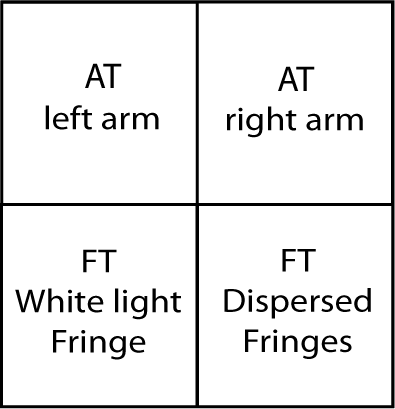
\includegraphics[width=0.2\textwidth]{Figures/Quad.png}
%{Two snapshots of BETTII's carbon fiber gondola and external optics. To the left, one early design is shown, without most of the holding structures for the optics. To the right, a more recent model is shown, with additional elements to connect the optics and to connect to the balloon train. This structure has exceptional thermal properties, and very high frequency vibration modes.}
\caption{Single H1RG with four quadrants.}
\label{fig:quad}
\end{center}
\end{figure}

%The FTU can operate over fields of view larger than the science channels, if the full quadrants of the H1RG are readout. However, as we look at the edges of the field of view, the aberrations will become a problem, especially in the FT. Our actual usable field of view will be determined after the optical design is completed and all issues are resolved.
%Working in the NIR gives us two advantages: first, we are not using the science photons and are not subject to the considerable background noise present at long wavelengths; second, we are naturally more sensitive to OPD: \textit{Achieving, even poorly, angle and fringe tracking in the NIR would guarantee a good science return}, since the long wavelengths of the science channels are naturally more forgiving than the NIR channels. However, for the fringe tracker to operate at this level, we must place more stringent requirements on the external optics (and structure) than would be required for the science channels alone.

\subsection{Angle tracker concept}\label{subsec:ANGLE}


The AT feeds an error signal to fast steering tip/tilt mirrors that compensate for any movement of the star with respect to a given location in each quadrant. In OBSERVE mode, we baseline a sensing frequency of 100 Hz, two orders of magnitudes faster than any expected external perturbation on our system.

We baseline simple centroiding algorithms and image motion sensing algorithms \citep{Hardy:1998ul}. As we continue work with the FTU testbed in the laboratory, we will investigate additional algorithm options to optimize the performance of the FTU.

%The algorithms used for identifying and tracking the guiding star are presently under investigation. To identify the guiding star, we might want to use a wide field of view and a star pattern-recognition software, similar to the one used for the star camera. For tracking, we will likely use simple centroiding algorithms along with image motion sensing algorithms.

The control architecture in OBSERVE mode is the following. The H1RG reads out only one small region of interest in each arm, located around the spot where we have driven the guide star, and generates an error signal. This signal is fed to the tip/tilts to correct the angle deviation through a simple control loop. The correction signal is also used by the siderostats and the azimuth control to correct the pointing of the overall gondola in azimuth and elevation, at a slower frequency, in order to maintain the tip/tilts near the center of their range. 

%Several options for the tip/tilt stages and actuators are still under investigation. Our baseline design uses Newport goniometer stages and piezo-actuators, although it is unclear if these will withstand the high frequency motion and the conditions at float. A vacuum chamber is presently under construction that will allow thorough testing of the candidates under adequate pressure and temperature conditions. 

\subsection{Fringe tracker concept}\label{subsec:FRINGETRACKER}
%\subsubsection{On the important role of a fringe tracker}
%BETTII's fringe tracker shares the optical train with the science interferometer, so it will monitor all the net OPD perturbations caused by the combination of pointing errors and any type of internal perturbations. It will also allow us to have an absolute phase reference. In addition, the FT ensures that ZPD always stays within the range of the CDL, so that we are properly scanning through ZPD for the whole field of view.

%The second aspect is that we see the 2$\um$ FT as a path forward to the future of free-flying interferometers. Enabling this type of technology would pave the way to a wide field of science experiments, that would benefit from a clear atmosphere (hence allowing long integration times) while still having relatively long baselines (good spatial resolution), a combination that is challenging on the ground because of atmospheric turbulence. Our FT has inherent interferometric resolution of $\lambda/B\sim$ 50mas, so one can imagine all sorts of science fields that would benefit from low-background, low phase-noise observations at these wavelengths. 

%However, making the FT work tightens all the requirements by an order of magnitude, since now we are constructing a free-flying, 2$\um$ interferometer with an 8m baseline, which needs to be robust to 100K of thermal shift between the environment in which it is aligned and the environment in which it will operate.

\subsubsection{Design details}

The bulk of the impact of the pointing errors on the OPD will be measured by the gyroscopes and the AT. This can be fed directly to the WDL in order to compensate for it, by converting the angular rate to a delay line speed, with appropriate coordinate system transformations. This approximately ``freezes" the fringe motion due to pointing errors.

However, this only gives us a blind, open-loop correction of the OPD since we have no feedback on what the actual OPD; we only know how much it varies due to pointing errors. The FT comes into play here by closing this loop and providing a direct measurement of the net OPD. We will use simple, robust schemes that operate fringe-scanning and fringe-tracking in order to find and keep the fringes in a known position. Note that for our science, \textit{it is only necessary to know where the 2 $\um$ fringes are, not necessarily to stay on the central fringe}.

\subsubsection{Fringe finding and tracking algorithms}

%Given the environmental conditions described in section \ref{sec:PERT}, the gondola will be subject to a sum of low-frequency sinewave motions that are generated by pendulation. Our control system (Benford et al. 2012, these proceedings) should be able to stabilize the gondola to better than 10 "/s. Taking this value as a maximum pointing drift in pure cross-elevation, it will make ZPD move at 400 $\um$/s in delay space, or 200 fringes/s. Although this is too fast for the H1RG to read and measure any fringe modulation, this rate can be estimated by the gyroscopes and the AT, and fed directly to the WDL through a PID loop.

%However, the above only gives us a blind, open-loop correction of the movement of ZPD. Although this ``freezes" the fringes, there could still be an offset between the actual position of our delay line and the real location of ZPD. There will also be an error due to non-ideal correction and estimation errors due to gyroscope drift, etc. The 2 $\um$ FT comes into play here, closing this loop. We will use simple, robust schemes that operate fringe-scanning and fringe-tracking in order to find and keep the fringes in a known position.  Hence, one can imagine a scheme where we scan back and forth through the fringe packet and interpolate the location of ZPD at each step.

%\begin{figure}[ht!]
%\begin{center}
%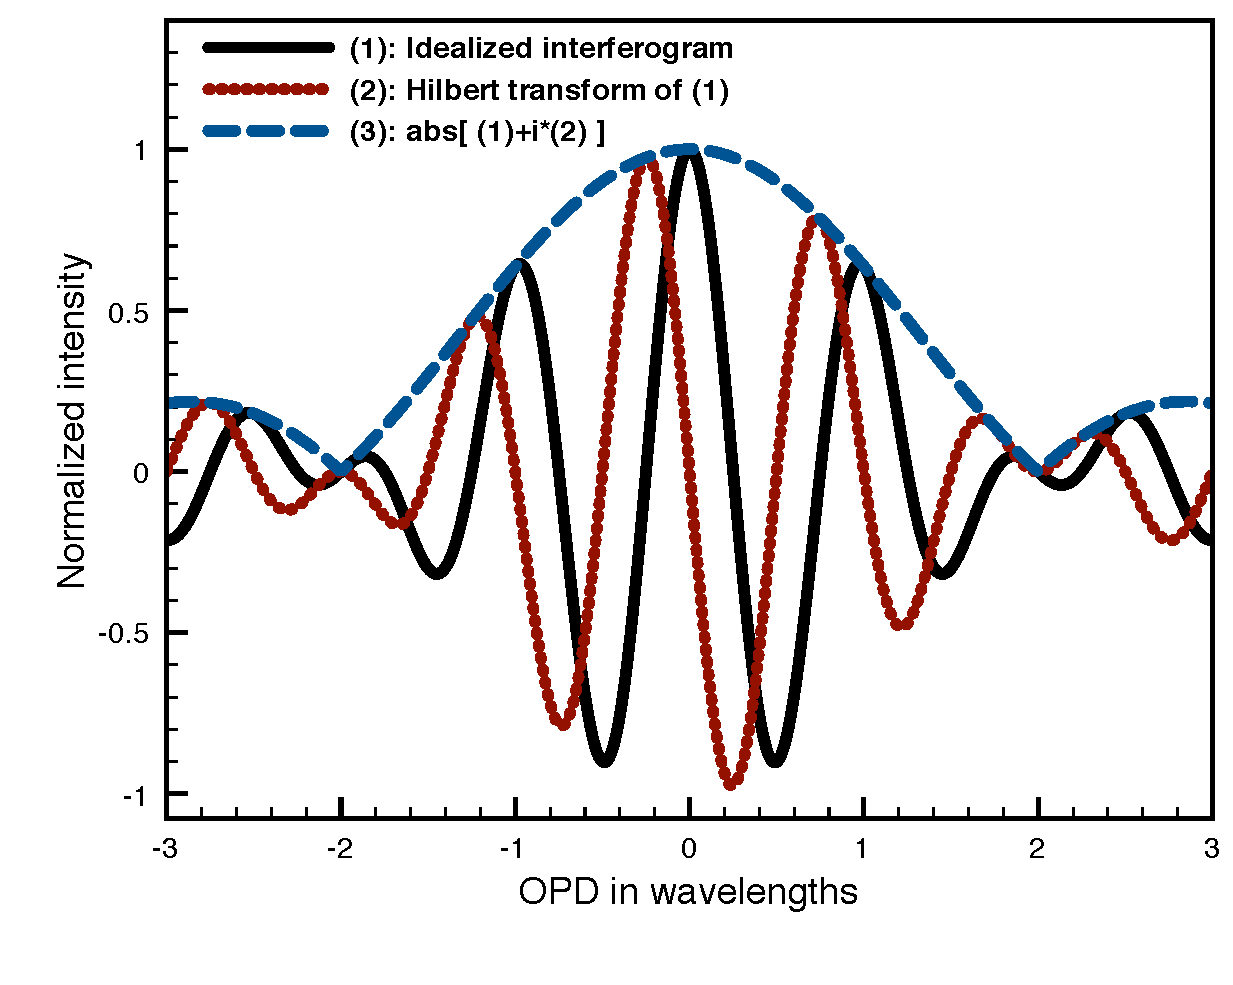
\includegraphics[width=0.5\textwidth]{Images/HT.pdf}
%\caption{Hilbert Transform of idealized interferogram.}
%{Two snapshots of BETTII's carbon fiber gondola and external optics. To the left, one early design is shown, without most of the holding structures for the optics. To the right, a more recent model is shown, with additional elements to connect the optics and to connect to the balloon train. This structure has exceptional thermal properties, and very high frequency vibration modes.}
%\label{fig:HT}
%\end{center}
%\end{figure}
We baseline a Hilbert transform algorithm to give us the fringe envelope, and a sliding-parabola fitting routine to give us the peak the envelope, which is a measure of the center of the fringe packet. The position of the WDL that corresponds to the center of the fringe packet is the point of ZPD. At this point we are sure that all net external OPD effects have been corrected, and now we can robustly interpret the movement of the CDL in the science instrument.

The Hilbert transform algorithm will be used for scans larger than the fringe packet, and in particular for initial determination of the fringe location. We baseline a version of the 4-bucket algorithm (also called ABCD \citep{Colavita:2010ce}) to lock on the fringes once we found them, with multiple backup options if that algorithm fails. This algorithm also uses the dispersed output to provide group delay information at a slower frequency \citep{Colavita:2010ce}.

Once we lock on the fringes, we make measurements of the OPD at 25~Hz (4 measurements at 100~Hz are required to make one estimation of the OPD). If the locking algorithm fails, we can use the Hilbert transform to scan back and forth through the fringe packet, determine the location of the envelope peak for each scan, and interpolate between scans. We can expect this algorithm to work at 1-3~Hz.

Hence in OBSERVE mode the WDL will implement two movements at once: the first has a slow frequency and large amplitude to follow gondola pendulation and mispointing, and occurs whether or not fringes are found with the 2~$\um$ FT; this uses the gyroscopes and AT signals to freeze the OPD. The second movement scans the OPD to look for fringes and lock on them once they are found. Residual errors from our gyroscopes and AT will likely prevent the WDL from being able to completely freeze ZPD for a whole scan duration: this will create dynamic variations of our 2~$\um$ fringe sampling when scanning for fringes.
%Note that during a given scan of the WDL (which always occurs on top of the broad motion that compensates for smooth pointing errors), there will be a residual error in our attitude rate estimation, as well as multiple other unpredicted perturbations. The error in the rate estimation will create a dynamic variation of the the effective sampling of our fringes, which can be seen, to first order, as a phase chirp. 
The Hilbert transform, although computationally heavier than other algorithms, is insensitive to sampling variations and inhomogeneities since it has an infinite bandwidth and affects all frequencies in the signal. The ABCD, on the other side, is a filter matched to one given sampling frequency, which is less appropriate to this problem.

%\subsubsection{Envelope determination by Hilbert transform}

%The Hilbert transform (HT) of a complex data sample consists in a multiplication by $-i\times\textrm{sign}(f)$ in the frequency domain. This has the effect of shifting all frequencies in the signal by $\pi/2$. In particular cosines are transformed to sines, and interferograms $I(\phi)=V(\phi)\cos(\phi)$ are transformed into $I_{\pi/2}(\phi)=V(\phi)\sin(\phi)$. The square envelope is estimated as $V^2(\phi)=I^2(\phi)+I_{\pi/2}^2(\phi)$. It is also interesting to note that the noise statistics are unchanged through the HT, so $I$ and $I_{\pi/2}$ have the same noise variance $\sigma^2_I$. The mean of the square envelope is connected to the interferogram's variance by: $\langle V^2\rangle = 2\sigma^2_I$. 




%\section{BASELINE INTERFEROMETRY FROM 35 KM ALTITUDE} \label{sec:PERT}
%\subsection{On the scientific potential of free-flying interferometers}\label{subsec:POT}
%Should I explain here all the ideas I have in case BETTII really works? (2$\um$ interferometry, astrometry, etc) Or should I keep it all a secret?

%BETTII's concept is inherited from proposed space missions SPECS (reference) and SPIRIT (reference), which featured movable baseline to provide extended UV coverage. BETTII's science goals are more modest, but the mission aims at paving the way for future balloon-borne and space-based interferometric missions. 

%If BETTII is a success, it opens up the possibilities of doing high resolution interferometry at long wavelengths that are inaccessible from the ground. In addition, if BETTII's fringe tracker works, it opens up many possibilities for near-IR interferometry. 

%We investigate some of the potential perturbations that are important for a NIR interferometer. Here, we focus on the effects of the atmosphere and the payload pendulum modes. Other perturbations, such as the ones caused by thermal gradients, are discussed in Benford et al., 2012 and Rinehart et al., 2012 (these proceedings). 

%\subsection{The environment at 35 km}\label{subsec:ENV}
%temperature, pressure; cite someone here
%At an altitude of 35 km the typical temperature is $\sim$220-230 K, the typical pressure is $\sim$0.01 bar, and the density of air is $\sim$0.02 kg.m$^{-3}$.
%The temperature is an important element because it will determine the dominant amount of far-infrared background radiation, by setting the temperature of the warm optics. It is expected that, over the course of one night ($\sim$8 hrs), the temperature of the optics will constantly be dropping, from $\sim$310 K at launch to $\sim$226 K at float, and that we will never reach thermal equilibrium.

%Using standard off-the-shelf computers, electronics, and actuators is challenging under these conditions, as they are typically neither designed for nor tested in this type of environment. Rinehart et al., 2012 (these proceedings) describe the test test chamber we are building to test the candidate hardware.

%The structure has exceptional properties, such as a lowest resonant mode above 20 Hz. To the best of our knowledge, there is no external perturbation that can excite structural modes at such a high natural frequency. There are several identified low-frequency pendulum modes that we describe briefly in section \ref{subsec:PENDULUM}, but these are all $<$0.5 Hz. Thus, in the design of BETTII and its fringe tracking unit, we work under the assumption that \textit{all high frequency vibrations will be excited by the payload itself}. Hence, a meticulous test plan will be used to robustly identify all sources of self-generated perturbations when BETTII is fully up and running in the lab. 

%For an interferometer, it is also important to consider other aspects of the environment, and in particular the stability of the overall system for the relevant time scales. Although measurements have been made at rather large scales (arcminute scale, see section \ref{subsec:PENDULUM}), there is very little literature about the stability of systems to the sub-arcsecond level. However, to the best of our knowledge, there is no physical mechanism to excite high-frequency ($>$10Hz), arcsecond-level gondola jitters. 

%\subsection{The atmosphere above the observatory}\label{subsec:ATMO}

%\subsubsection{Fried parameter and coherence time}
%There has been extensive studies on atmospheric turbulence and its impacts on the performance of ground-based telescopes\cite{Hardy:1998p2181}. The atmosphere distorts the wavefronts  due to inhomogeneities in temperature which in turn create inhomogeneities in the index of refraction of the air along the line of sight. As two telescopes separated by some distance look at the same target on the sky, the atmosphere above each these telescopes is slightly different. As a result the two wavefronts will have residual piston errors (in addition to other effects), that can be changing rapidly and considerably complicate the fringe tracking process.

%Usually, the level of atmospheric disturbances is represented by a characteristic turbulent scale size, $r_0$, also called the Fried parameter\cite{Fried:1966p2197}, which can be understood as the aperture size over which the mean square wavefront error is 1 square radian\cite{Hardy:1998p2181}. The Fried parameter synthesizes the effect of the integrated variations over the light path within the atmosphere. On the ground $r_0$ is usually less then a few tens of centimeters in the optical and NIR, even at the best facilities.

%However, above the tropopause, winds are much more stable and atmospheric turbulence has decreased by orders of magnitude. At 30 km and above, there is very little atmosphere left and its integrated contribution on the wavefront is now negligible. We can estimate what $r_0$ will be, as well as how fast our system needs to operate in order not to be affected by atmospheric phase noise between our two apertures separated by $B=8$ m. We use models\cite{Perlot:2009p1124} that are based on space-based measurements of stellar scintillation through the atmosphere\cite{Gurvich:2007p1117} to determine the temperature gradient through the upper atmosphere. The variation in index of refraction is directly related to the temperature structure. We use $C_n^2$ as the refractive index structure parameter\cite{Hardy:1998p2181}. We use the following model for the upper atmosphere:
%\begin{equation}
%C_n^2(h) = \left[2.7\times 10^{-4}e^{-h/H_0}\right]^2\times 10^{-10}e^{-h/H_1},
%\end{equation}
%where $H_0$ is the traditional atmospheric scale height, $H_0\sim 7$ km, and $H_1=10$ km\cite{Perlot:2009p1124}. We can now write\cite{Hardy:1998p2181}:
%\begin{equation}
%r_0(\theta) = \left[0.423\left(\frac{2\pi}{\lambda}\right)^2\frac{1}{\cos(\theta)} \int_{\textrm{alt}}^{\infty} C_n^2(h)dh\right]^{-3/5},
%\end{equation}
%where $\theta$ corresponds to the angle between the line of sight and the zenith. One obtain a typical cell size $r_0\sim 12$ km for 45 degrees elevation and an altitude alt=35 km. The characteristic frequency of the atmospheric turbulence is called the Greenwood frequency\cite{Hardy:1998p2181}, and an approximation of it is:
%\begin{equation}
%f_G=0.427\frac{v}{r_0},
%\end{equation}
%with $v$ the wind speed, that we can take as being $\sim$ 6 m.s$^{-1}$. We obtain a typical Greenwood frequency $\sim 0.2$ mHz with the same model used before\cite{Perlot:2009p1124}. 

%One other important consideration is the typical coherence time, that is, the integration time after which the rms wavefront error between both apertures has reached 1 rad. We use\cite{Colavita:1999p153} $T_c=0.815r_0/v$, and we find that $T_c\sim 1600$ s. 

%To test the robustness of these parameters, let's assume that the models underestimate the integrated amount of atmospheric turbulence by three orders of magnitude. In that case, $r_0 \sim 200$ m, $f_G=10$ mHz and $T_c=25$ s, which are still very comfortable values to design a proper instrument. We conclude that \textit{even if the float conditions are significantly worse than expected, the atmosphere does not provide any fundamental impediment for balloon-borne, NIR interferometry.}



%This demonstrates that balloon-borne interferometers are not subject to atmospheric turbulence perturbations over any reasonable timescale and thus do not require any adaptive optics system, even at short wavelengths ($r_0$ scales as $\lambda^{6/5}$). This is a great advantage for balloon-borne facilities trying to achieve baseline interferometry, but it is also excellent for regular telescopes trying to undertake observations that want to minimize seeing (which also depends on $r_0$).

%\subsubsection{Absorption bands in the NIR}
%{Two snapshots of BETTII's carbon fiber gondola and external optics. To the left, one early design is shown, without most of the holding structures for the optics. To the right, a more recent model is shown, with additional elements to connect the optics and to connect to the balloon train. This structure has exceptional thermal properties, and very high frequency vibration modes.}
%We ran models using MODTRAN of the atmospheric transmission both at a usual 4 km altitude, where one can distinguishes J, H, K bands, and at balloon altitude. At float, the transmission is excellent and the wavelength bands of our instruments are not constrained by the atmosphere.

%\subsection{Pendulum modes} \label{subsec:PENDULUM}
%The previous sections indicate that the atmosphere is not going to be a limitation in the design of a 2 $\um$, 8-m baseline interferometer. However, the more significant issue is the lack of complete control of the gondola.
%Indeed, the large-scale, low-frequency motions that are observed\cite{Fixsen:1996p737} are due to the geometric configuration of the balloon-payload assembly. As the payload hangs from a long ladder attached to a large and massive balloon, the geometry implies natural pendulum modes that have been measured by several balloon missions\cite{Fixsen:1996p737}. These were shown to be fairly predictable even with simple models. The periods of these modes range between $\sim$ 2 s and $\sim$ 30 s, and the amplitudes of up to $\sim$ 5-10 arcminutes. 

%The pendulum modes are excited right after ascent, as well as after each large slew. Since the coupling to the ambient, low-density air is very low, these modes are only slowly damped (they have typical $Q$ factors of about 30) and thus one needs to be actively controlling them to stay pointed.
%Despite the large amplitudes of these modes, previous balloon missions have shown the ability to stay pointed at a given target better than an arcminute, and we will use this figure for design purposes. A preliminary, rigid-body model of BETTII and its basic control system model already provides better results for the moment, but several parameters still remain to be tuned.

%While BETTII will achieve arcsecond-level angular resolution, this does not require gondola pointing at the arcsecond level.  By using an interferometer, pointing errors can be directly translated to OPD errors (see Fig. \ref{fig:pendulum}), and can be taken out in a delay line. In theory, therefore, BETTII partially decouples the resolution of the instrument from the gondola pointing, eliminating the requirement for sub-arcsecond pointing stability.


%\begin{figure}[ht!]
%\begin{center}
%\includegraphics[width=0.4\textwidth]
%{Images/BETTII_Pendulation_CrossElevation.png}
%{Two snapshots of BETTII's carbon fiber gondola and external optics. To the left, one early design is shown, without most of the holding structures for the optics. To the right, a more recent model is shown, with additional elements to connect the optics and to connect to the balloon train. This structure has exceptional thermal properties, and very high frequency vibration modes.}
%\caption{A cross-elevation pendulum mode changes the OPD by making one arm slightly longer than the other. With an 8 m baseline, 1" of pointing error in the cross-elevation direction corresponds to $\sim$40 $\um$ of OPD. To compensate for this effect, BETTII needs to control both azimuth and elevation. Note that pendulum modes in the elevation direction do not affect the OPD. These are corrected by the siderostat elevation only.} 
%\label{fig:pendulum}
%\end{center}
%\end{figure}

%\subsection{Thermal effects} \label{subsec:THERMAL}
%The thermal environment of the gondola needs to be considered carefully, and is one of the heaviest modelling efforts. Although the temperature of the air can be expected to be uniform across the gondola, multiple components will have a deviation from ideal and could create challenging thermal gradients. In particular, as all the electronics, batteries and computers are embedded in the central aluminum section of the gondola, there will be a natural outward thermal gradient that will need to be modelled and potentially controlled.
%In addition, there will be the natural gradient between the bottom of BETTII, which sees the warm Earth, and the top of BETTII, which sees the very cold space. Although this is a symmetrical gradient in that it will affect both arms the same way, we are still planning on having a large mylar shield under the payload. Thermal gradients can get more complicated if the Sun is up, but we design BETTII to have nominal operations during the night. The effect of the Sun in terms of thermal effects and in terms of the star camera sensitivity will be modelled later down the road.

%The structure will shrink of several hundreds of microns over the course of the flight before it reaches thermal equilibrium. Although this can be very problematic for OPD purposes, the truss has excellent symmetry and thus we can expect very little differential motion between the two sides. This is the result of an on-going effort to design the system as symmetrical as possible, so self-generated perturbations and thermal gradient impact both arms in the same way.



%\subsection{Cosmic rays}
%One other downside of being that high up in the atmosphere is that we are not protected from cosmic rays as we are down on the ground. This complicates the software design as it needs to be as robust as possible to glitches induced by cosmic rays. 
 
%\subsection{Other perturbations} \label{subsec:OTHERPERT}
%Other types of perturbations are discussed in Rinehart et al and Benford et al. (these proceedings). Among them, the thermal behavior of the gondola is critical for long-term optical stability. The momentum wheel assembly used to control the azimuth of the payload is expected to inject high-frequency vibrations in the gondola, and they will be thoroughly measured in the lab. However, BETTII is designed to be robust to perturbations that occur symmetrically in both arms, which 
%Among the other significant perturbations that we anticipate are the ones that could be created by the momentum wheels that we are using to control the azimuth of the payload. Two wheels are used along with stepper motors and can inject high-frequency perturbations into the whole gondola, if the wheel assembly is not properly isolated from the rest of the structure, or if the perturbations propagate differently in both arms. Although the details of these perturbations are still to be worked out, this is in principle testable on the ground.

%Other events, such as dropping a ballast and temperature-induced structural ``popping", will have less predictable effects. It will be natural for BETTII to have an on-board calibration procedure that resets the position of zero optical path difference within the gondola.

%\subsection{The importance of synchronization and the one-clock paradigm}
%Since the perturbations are self-generated, it is of paramount importance to synchronize every moving and sensing element on the gondola. In order to achieve this challenge, we are working with a one-clock paradigm, which has proven to work on previous balloon missions undertaken by members of the team\cite{Fixsen:1996p737}. This consists in having one single master clock for the whole payload, which is distributed to every subsystem after being divided by an integer number. Although this is possible in principle, it creates difficulties as we are considering buying off-the-shelf actuators and sensors, which sometimes come with their own electronics and sometimes their own clock.

%\subsection{Autonomy of the payload}
%Although this is not strictly speaking a feature of the environment, it is important to note that two-way communication with the payload will be limited. The up/downlink will actually change as the payload drifts away from the launch facility. It will not be possible, for example, to stream down large quantities of data, or completely upload a new version of the flight software. This is possibly where BETTII differs the most from ground-based interferometers, in the sense that it needs to be able to make a lot of decisions on its own, and should be baselined to operate completely autonomously by default. In practice, we will have ways to make executive decisions such as switching between operating modes, especially for our first flight (e.g., if we don't find NIR fringes, etc). This is important to note, as \textit{we do not design BETTII to be a remote-controlled instrument}, but instead a real autonomous payload that will implement a pre-determined flight plan and can decide whether or not it can move on to the next step.





\section{FTU PARAMETERS AND SENSITIVITY}\label{sec:PARAMS}
\subsection{Top-level Parameters}
\begin{table}[!ht]
\begin{center}
\caption{FTU parameters. }
\label{tb:FTUparams}
\begin{tabular}{|c||c|c|}
\hline 
Parameter & Angle Tracker & Fringe tracker \\ 
\hline 
\hline
Central wavelength $\lambda_0$ & 1.25 $\um$ & 2 $\um$ \\ 
\hline 
Bandpass $\Delta\lambda$ & 0.5 $\um$ & 0.8 $\um$ \\ 
\hline 
Plate scale & 0.6"/px & 1"/px \\ 
\hline 
Airy disk diameter & 2~px & 2~px \\ 
\hline 
Throughput efficiency & $\sim$35\% & $\sim$35\% \\ 
\hline 
Integration time per read & 10 ms & 10 ms \\ 
\hline 
Required performance & 0.1" & 1 $\um$ \\ 
\hline 
Range & 3' (on the sky) & 1 cm \\ 
\hline 
Minimum step size & 0.05" (on the sky) & 0.5 $\um$ \\ 
\hline 
Nominal sensing frequency & 100 Hz & 25 Hz \\ 
\hline 
\end{tabular} 
\end{center}
\end{table}

%The interferometric visibility specification is an on-going debate. We are presently designing the system to provide a  minimum visibility of $V=0.25$. We describe in section \ref{subsec:VIS} the details of the visibility budget.
The top-level design parameters are gathered in Table \ref{tb:FTUparams} for both the AT and the FT in a nominal OBSERVE mode.
The throughput efficiency assumes 12 mirror reflections with 99\% reflectivity, a detector quantum efficiency of 0.7, and about 55\% of additional loss due to dichroics and bandpass filters. The sensing frequency is the frequency at which we track the angular deviation (for the AT) or the OPD variations (for the FT). For the FT, if we can never lock on fringes, we can track them with the Hilbert transform at $\sim~1-3$~Hz.


\subsection{Background noise}\label{subsec:Noise}
At 2~$\um$, the dominant background noise is caused by the atmospheric airglow, generated by the OH lines at $\sim$~90~km altitude\cite{Hofmann:1977p2231}. Hence, our balloon experiment will be subject to this noise just like ground facilities. Although there has been inconsistency in the literature on the atmospheric radiance at 2.4~$\um$ \citep{Matsumoto:1994io,Mandolesi:1998wt} we use a conservative value for the radiance over both our bands, of $R_\textrm{atmo}=10$ nW.cm$^{-2}$.sr$^{-1}$. This corresponds to approximately 500 photons per second in the AT and 1600 photons per second in the FT. 

Since the AT and FT read out at 100 Hz in OBSERVE mode, these noise levels have standard deviations of 2 and 4~e$^{-}$~rms respectively, which will be negligible compared to the H1RG read noise of $\sigma_\textrm{CDS}$=18~e$^{-}$~rms. 

Other sources of noise of NIR background noise have been investigated, but none will have a significant contribution. Hence, the detector read noise will be our limiting factor for faint stars.

\subsection{Atmospheric effects}

\subsubsection{Transmission}
Balloon altitudes provide significantly better atmosphere transmission in the NIR wavelength region, compared to ground observatories. Fig. \ref{fig:trans} illustrates this difference using a modelling software called MODTRAN. The transmission from an altitude of 4~km shows transmission windows (J, H, K bands) that would limit the design of a ground-based interferometer. At float, the bands are not limited by the atmospheric transmission and thus we can use larger bands than the traditional J, H and K in order to optimize our photon signal.

\begin{figure}[ht!]
\begin{center}
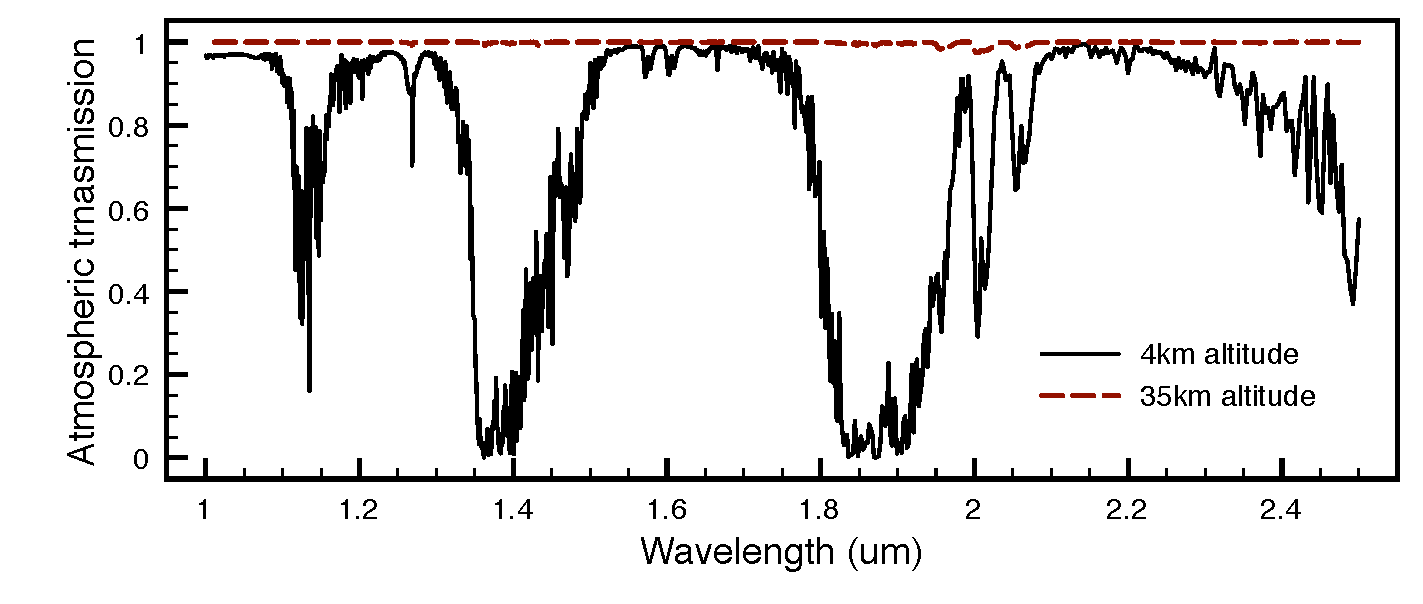
\includegraphics[width=0.6\textwidth]{Figures/trans.pdf}
\caption{Model atmospheric transmission}
\label{fig:trans}
\end{center}
\end{figure}

\subsubsection{Phase noise}

There has been extensive studies on atmospheric turbulence and its impacts on the performance of ground-based telescopes \citep[e.g.,][]{Hardy:1998ul}. The atmosphere distorts the wavefronts  due to inhomogeneities in temperature which in turn create inhomogeneities in the index of refraction of the air along the line of sight. As two telescopes separated by some distance look at the same target on the sky, the atmosphere above each these telescopes is slightly different. As a result the two wavefronts will have arrival time differences, that can be changing rapidly and considerably complicate the fringe tracking process. For BETTII's FTU, it is important to check if the atmospheric noise has significant impact on our fringe tracking capability.

Usually, the atmospheric disturbances are represented by a characteristic turbulent scale size, $r_0$, called the Fried parameter \citep{Fried:1966tk}, which can be understood as the aperture size over which the mean square wavefront error is 1 square radian \citep{Hardy:1998ul}. The Fried parameter synthesizes the effect of the integrated variations over the light path within the atmosphere. On the ground, $r_0$ is usually less than a few tens of centimeters in the optical and NIR, even at the highest facilities.

However, above the tropopause, winds are stable and atmospheric turbulence has decreased by orders of magnitude. At 30 km and above \citep{Perlot:2009jqa}, there is very little atmosphere left and its integrated contribution on the wavefront is nearly negligible. We use models for the upper atmopshere \citep{Perlot:2009jqa} to give us $C_n^2$, the refractive index structure parameter \citep{Hardy:1998ul}:
\begin{equation}
C_n^2(h) = \left[2.7\times 10^{-4}e^{-h/H_0}\right]^2\times 10^{-10}e^{-h/H_1},
\end{equation}
where $H_0$ is the traditional atmospheric scale height, $H_0\sim 7$ km, and $H_1=10$ km is another scale height\cite{Perlot:2009p1124}. This is a critical parameter needed to determine the Fried parameter \citep{Hardy:1998ul}:
\begin{equation}
r_0(\theta) = \left[0.423\left(\frac{2\pi}{\lambda}\right)^2\frac{1}{\cos(\theta)} \int_{\textrm{h=35~km}}^{\infty} C_n^2(h)dh\right]^{-3/5},
\end{equation}
where $\theta$ corresponds to the angle between the line of sight and the zenith. At $\lambda=2~\um$, one obtains a typical cell size $r_0\sim 12$ km for 45~degrees elevation and an altitude of 35~km. The characteristic frequency of the atmospheric turbulence is called the Greenwood frequency\cite{Hardy:1998p2181}, $f_G\sim0.427 v /r_0\sim 0.2$ ~mHz, where $v\sim 6$~m.s$^{-1}$ is the wind speed.

One other important consideration is the typical coherence time for a two-telescope interferometer\cite{Colavita:1999p153}, $T_c\sim 0.815r_0/v\sim 1600$~s. This corresponds to the integration time during which the rms wavefront error about the interval mean has reached 1~radian~rms.

With a baseline $B\ll r_0$, an operating FT frequency of 1~Hz $\gg f_G$ in the worst case (25~Hz nominal), and integration times of 10~ms $\ll T_c$, our system is very robust to atmospheric phase noise. In order for the phase noise to degrade our performance, $\int_{\textrm{h}}^{\infty} C_n^2(h)dh$ would have to be larger than the model by five orders of magnitude, which would give $r_0\sim 12$~m, $f_G=0.2$~Hz, and $T_c=1.6$~s. \textit{We conclude that the atmosphere is not a limitation for balloon-borne, NIR interferometry.}


\subsection{Faintest detectable star and projected performance}\label{subsec:FAINTEST}
Using the background noise levels described in section \ref{subsec:Noise}, we can estimate the limiting magnitude of the AT and the FT. We pick J-magnitude reference points for the AT band, and K-magnitude reference point for the FT band, a reasonably conservative estimate since our guide stars will usually be brighter at shorter wavelengths, and our bands extend shortward of the regular J and K bands.

\begin{table}[!ht]
\begin{center}
\caption{Limiting magnitudes }
\label{tb:LimMag}
\begin{tabular}{|c||c|c|}
\hline 
Parameter & Angle Tracker & Fringe tracker \\ 
\hline 
\hline
Specified SNR per 10 ms read & 10 & 10 \\ 
\hline 
Minimum flux density (mJy) & 70 & 70 \\ 
\hline 
Limiting Magnitude & 10.9 (Jmag) & 10 (Kmag)\\ 
\hline 
\end{tabular} 
\end{center}
\end{table}

Table \ref{tb:LimMag} shows the limiting magnitudes for the desired SNR ratio. We baseline a SNR of 10 on the flux estimate for the AT. We are confident that it will allow the required sub-pixel centroid accuracy, although this will be robustly assessed after thorough testing in the next couple of months.

%Although the research on algorithms for centroiding and image motion is still ongoing, we baseline a SNR of 5 on the flux estimate in the AT, which likely will be able to provide a sub-pixel centroid accuracy.

The SNR of 10 on the flux estimate for the FT is derived from a specified interferometric SNR of 2.5 and a visibility $V=0.25$. We are confident that fringe tracking can be achieved with this SNR, based on our experience in the lab described in section \ref{sec:TESTBED}.

\subsection{Visibility budget}\label{subsec:VIS}

The visibility budget for the FT fringes is shown in table \ref{tb:Budget}. The static contributors to the budget need to be met at all times, and are composed of the differential wavefront errors (WFE) due to mirror surface quality and system misalignments, the amplitude mismatch between the two beams, the polarization effect and the pupil shear at beam combination \citep{Lawson:2000vf}. The differential WFE effect from misalignments is by far the strongest contributor to the budget. 

Dynamical effects will also degrade the visibility, as the FT tries to integrate the interferometric signal. Hence these need to be met every 10~ms, our typical integration time. The uncorrected OPD corresponds to the residual OPD after the WDL compensates for pointing errors. This is the combination of an estimation error (the gyroscopes/AT are not perfect) and a control error (the WDL will not correct perfectly the signal from the gyroscopes/AT). This will be met if the WDL can correct the real pointing-induced OPD error to better than $\sim 15~\um/\textrm{s}$, or 0.4"/s in equivalent pointing error. Estimation of the angular rate to this precision is achievable by both the gyroscopes and the AT. The differential tip/tilt corresponds to the angle between the two incoming beams, and determines how well the AT needs to achieve centroiding. This requirement feeds through the AT, and is rather loose as its contribution is small. Finally, the unallocated piston jitter acts as our margin. It is possible, for example, that some perturbations such as the one created by the momentum wheels can excite asymmetric vibrations that would hence create some piston jitter over 10~ms time scales.

%The pure piston jitter acts as our margin, since there is no predicted perturbation that should create piston jitter at $>$100~Hz. The error in azimuthal mispointing correction describes how well we need to estimate and compensate for the azimuth rate. The WDL needs to achieve an OPD compensation equivalent to this level. Assuming a perfect WDL with infinite bandwidth, this is equivalent to saying that our attitude rate estimate needs to be better than 0.4"/second, which will be possible with our gyroscopes and our AT. By far the largest contributor to our visibility loss is the differential wavefront error (WFE), due both to the mirror surface quality and to inaccuracies in alignment of the optical system. While the mirror WFE budget is met by having 12 mirrors with $\lambda/20$ surface quality at optical wavelengths, meeting the other differential WFE budget is very challenging and is discussed in section \ref{subsec:SENSITIVITY}. The differential tip/tilt allocation tells us how well we need to overlap the two Airy disks, and this requirement is soft since the impact in the visibility loss is less. The amplitude mismatch is expected to be achieved easily, as is the polarization effect. The pupil overlap allocation is challenging because it is strongly dependent of where we put the pupil in the FTU. Satisfying this budget and appropriately all effects is still an on-going effort and will likely require several more iterations.

\begin{table}[!ht]
\begin{center}
\caption{Visibility budget}
\label{tb:Budget}
\begin{tabular}{|c||c|c|c|c|c|}
\hline 
Term & Symbol & Alloc. & Units & Effect on visibility \citep{Lawson:2000vf} & $V_\textrm{loss}$  \\ 

\hline 
\hline 
\multicolumn{6}{|c|}{\textbf{Static contributors}} \\ 
\hline
WFE in mirror surface & $\sigma_\textrm{WFE,mir}$ & 0.1 & $\um$ rms & $\exp(-[2\pi\sigma_\textrm{WFE,mir}/\lambda]^2)$ & 0.9 \\ 
\hline 
Other differential WFE & $\sigma_\textrm{WFE}$ & 0.3 &$\um$ rms & $\exp(-[2\pi\sigma_\textrm{WFE}/\lambda]^2)$ & 0.4 \\ 
\hline 
Amplitude mismatch & $R$ & 90 & \% & $2/(R^{1/2}+R^{-1/2})$ & 0.99 \\ 
\hline 
Polarization effect & $\theta$ & 12 & degrees & $\cos(\pi\theta/180/2)$ & 0.99 \\ 
\hline 
Pupil area overlap & $f_\textrm{overlap}$ & 95 & \% & $f_\textrm{overlap}$ & 0.95 \\ 

\hline
\hline
\multicolumn{6}{|c|}{\textbf{Dynamical contributors (valid for each 10~ms integration)}} \\ 
\hline
Uncorrected OPD & $\sigma_\textrm{mp}$ & 0.15 & $\um$ rms & $\exp(-[2\pi\sigma_{\textrm{mp}}/\lambda]^2)$ & 0.8 \\ 
\hline 
Differential tip/tilt & $\sigma_\textrm{tt}$ & 0.1 & asec rms & $2J_1(\pi D\sigma_\textrm{tt,rad}/\lambda)/(\pi D\sigma_\textrm{tt,rad}/\lambda)$ & 0.98 \\ 
\hline 
Unallocated piston jitter & $\sigma_\textrm{piston}$ & 0.1 & $\um$ rms& $\exp(-[2\pi\sigma_\textrm{piston}/\lambda]^2)$ & 0.9  \\ 
\hline 
\hline
\multicolumn{4}{|r|}{\textbf{Total visibility over 10~ms}} & $\prod (V_\textrm{loss})$ & 0.25 \\ 
\hline

\end{tabular} 
\end{center}
\end{table}

\subsection{Alignment sensitivity study: the tough spots of BETTII}\label{subsec:SENSITIVITY}

The visibility budget for the FT drives the alignment sensitivity analysis, which tells us how well we need to align the optics, and how well we need to maintain their relative positions and angles. While the complete details of this analysis are beyond the scope of this paper, it has led to several important points worthy of mention. First, the strongest  requirements are all on the external optics, which are also more challenging to align and stabilize because of the flight environment to which they will be exposed.

The most challenging alignment is between the primary and the secondary mirrors. With a 20:1 beam compression, aberrations created by position shifts of the secondary are dramatic. Although the design is very symmetric and thus will generate mostly symmetric perturbations in both arms, the fields are flipped before entering the telescopes and thus symmetrical perturbations will not create symmetrical WFE. Symmetrical WFE would have no effect on the visibility as it would degrade the wavefront identically in both arms. 

We are minimizing these effects by implementing a homologous design, building the primary, secondary, and supports from a single material, and actively maintaining the structure at a uniform temperature to within 0.5~K.

Alignment effects on the visibility, both in pupil shear and differential WFE, are field dependent. In the middle of the field, the FT has a sweet spot where it is less sensitive to several misalignments. Hence, we choose to put our guide star nominally at the center of the FTU field of view. This is allowed since, even if the science target is pushed to the edges of the field of view, the effects of these misalignments are not as severe on the science visibility, due to the long wavelength of the science instrument.


%Our idea to mitigate this effect is to build the whole primary-secondary assembly out of aluminum, and run a liquid through the assembly in order to keep it isothermal. As the temperature changes while staying isothermal across the assembly, the latter will contract in a homologous fashion, thus not creating wavefront errors.



\section{A fringe-tracking testbed} \label{sec:TESTBED}
\subsection{The challenge of testing BETTII on the ground}
BETTII poses several challenges for system-level ground testing. In particular, the FT is very hard to test due to its sensitivity to atmospheric effects, both over 8~m in the lab, and even more if we look at an astronomical target through the turbulent atmosphere. Our hardware cannot accommodate the very short interferometric coherence time that we will have both in Greenbelt, Maryland and at the balloon launch facility in Texas or New Mexico. 


Full-system testing of the FTU is a problem, so a comprehensive test plan was developed for each subsystem. As a start, a first generation testbed was built out of hardware reused from another project. This effort was done in parallel to the FTU design phase and sensitivity analysis. The testbed was designed to gain experience with fringe tracking algorithms. We describe its concepts and results in the following sections.


%\subsection{A testbed to develop OPD determination algorithms}\label{subsec:TESTBED}
\subsection{Description}
A schematic and picture of the testbed is shown Fig. \ref{fig:layout}; it is essentially a traditional Mach-Zehnder interferometer at optical wavelengths. A halogen white light source is fed to a pinhole and collimated before it is injected in the interferometric core. It is split once, after which each arm goes through an independently controlled delay line. The two beams are then recombined, one output is directly imaged, and the second is dispersed then imaged. 

\begin{figure}[ht!]
\begin{center}
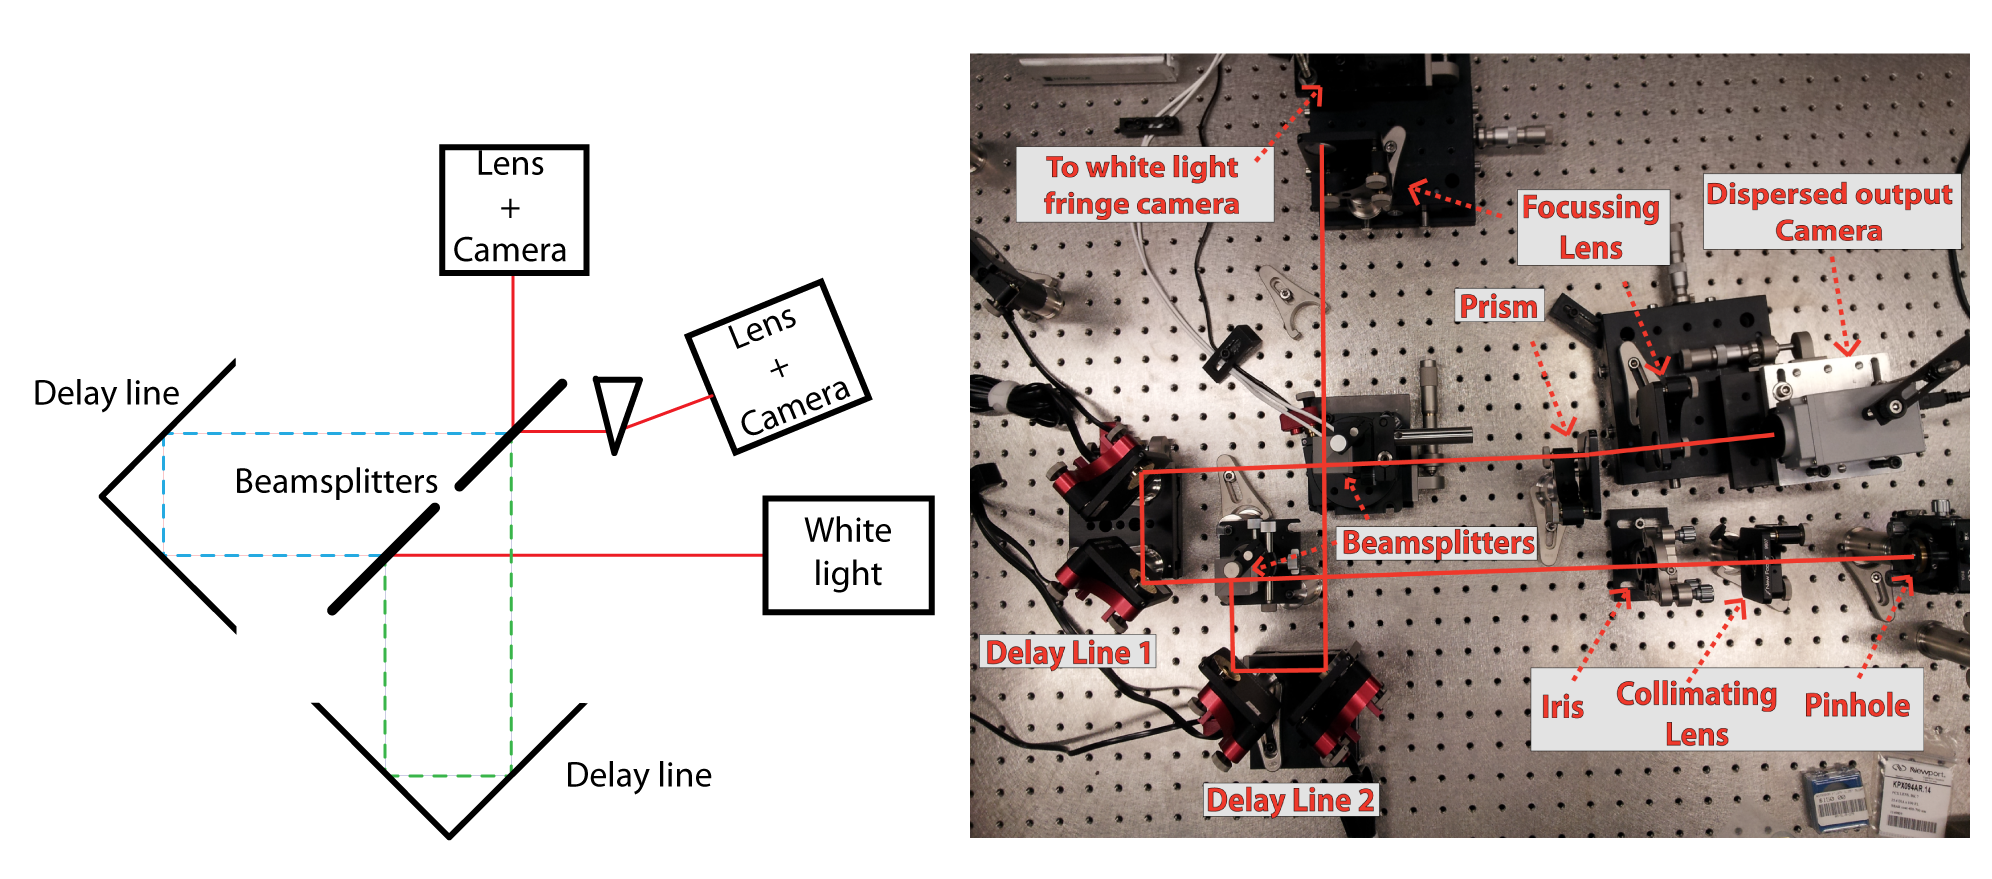
\includegraphics[width=0.8\textwidth]{Figures/layout.png}
%{Two snapshots of BETTII's carbon fiber gondola and external optics. To the left, one early design is shown, without most of the holding structures for the optics. To the right, a more recent model is shown, with additional elements to connect the optics and to connect to the balloon train. This structure has exceptional thermal properties, and very high frequency vibration modes.}
\caption{Optical layout, schematic and picture}
\label{fig:layout}
\end{center}
\end{figure}

Multiple filter setups are available for this testbed, but we mostly use the 20\% (618$\pm$60~nm) and 50\%  (800$\pm$200~nm) bandpass setups. The step size is about 60~nm. Note that we did not spend extensive efforts trying to align the interferometer to optimize the visibility. In particular, there are residual misalignments, differential WFE, and intensity mismatch that create a constant bias to the visibility. However, since we are only interested in the location of the peak center, optimizing the visibility is not be a priority for this first-generation testbed. In addition, we have not incorporated any absolute encoder yet.

\subsection{OPD measuring algorithms}
Three main algorithms have been explored, A, B, and C. A and B use interferogram scans several times the size of the fringe packet to find the peak location. Algorithm A computes the Hilbert transform of the interferogram, obtaining the fringe envelope function squared. The peak is identified after smoothing the envelope and using a sliding parabola fit. This method is insensitive to step size errors. The two regimes of operation are a high-SNR mode, where SNR~$\sim$~85, and a low-SNR mode with SNR~$\sim$~3 (see Fig \ref{fig:FirstScan}). 

\begin{figure}[ht!]
\begin{center}
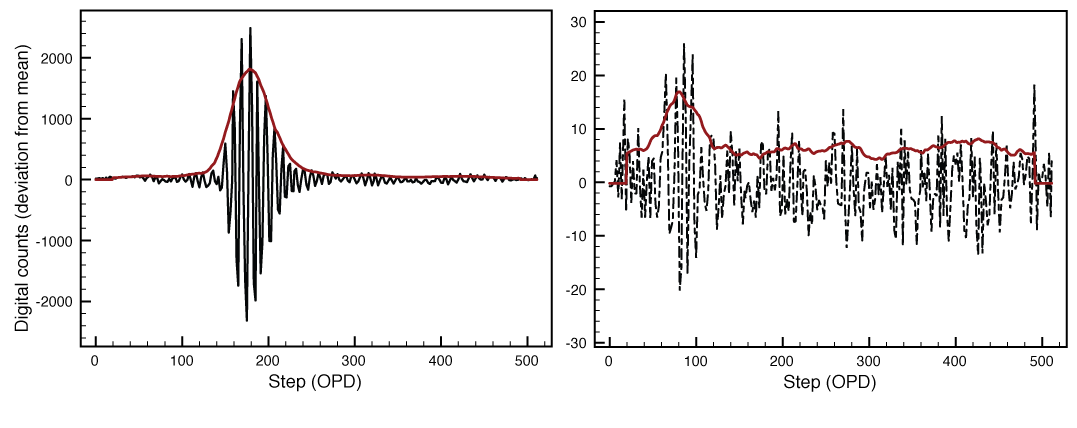
\includegraphics[width=0.8\textwidth]{Figures/FirstScan2.png}
%{Two snapshots of BETTII's carbon fiber gondola and external optics. To the left, one early design is shown, without most of the holding structures for the optics. To the right, a more recent model is shown, with additional elements to connect the optics and to connect to the balloon train. This structure has exceptional thermal properties, and very high frequency vibration modes.}
\caption{512 steps interferograms obtained under two regimes: SNR $\sim 85$, left; SNR $\sim 3$, right. The line above each interferogram corresponds to the smoothed envelope obtained with the Hilbert transform.}
\label{fig:FirstScan}
\end{center}
\end{figure}

Algorithm B uses the phase term in the Fourier transform of the interferogram \citep{Pedretti:2004ti}. This algorithm is sensitive to step size errors, as they change the location of the signal peak in Fourier space. Hence, the interferogram peak location is extracted by averaging the phases in the FFT over a broad range of bins. The bins that do not contain any signal will see their phases average out.

Both algorithms scan through the fringe packet, compute an identified center, and feed it back to a control loop with unity gain. The location of the next scan window is set to put the identified peak at the center of the window. We use the estimated squared visibility as our metric for successful tracking. For example, when the visibility suddenly decreases significantly from one scan to the other, we consider that we have lost the fringes. Our ability to track the fringes depends on the size of the scan window, which in turn determines the frequency at which we can track, provided a set integration time per data point.

Algorithm C implements dispersed fringe tracking over short $\sim 2$-wave scans around the central fringe. It computes the phase using the Hilbert transform in each wavelength channel (each detector pixel along the dispersion direction), and computes the slope of the phases with respect to wavenumber. The center of the next scan window is adjusted by using the measured slope times some control gain.

\subsection{Results}

\subsubsection{Description of the fringe tracking loop}
Our nominal fringe packet is about 80 steps wide ($\sim 4.8~\um$), so we choose a nominal scan size of 256 steps. We read these interferograms at 200 steps per second, which gives us a tracking frequency of a little less than 1~Hz, similar to what BETTII could have if the ABCD algorithm does not work. The peak is identified robustly through algorithms A and B simultaneously, and throws a flag if the two results are very different. The error signal is the difference between the identified peak location and the center of the scan window. This signal is fed back with unity gain in order to adjust the next scan. The control loop contains a two-point moving average on the error signal for each actuator direction. This allows proper treatment of the hysteresis/backlash and of linear changes in OPD, which are both dependent on the direction the actuator is moving.

\subsubsection{Peak estimation results}
We use A and B to estimate the location of the peak of the envelope in all scans. Both algorithms estimate the same peak location to within 3~steps~rms over multiple runs of 50 scans in the high-SNR regime. In the low-SNR regime, the two algorithms deviate of 5.5~steps~rms. This effectively corresponds to about half a wavelength of estimation error between scans, and we take this as our uncertainty on the real position of ZPD. This will be more robustly determined once we obtain absolute encoders. 

\subsubsection{Effects of hysteresis and backlash}

The actuators in the present testbed have significant hysteresis and backlash. With no absolute encoder, we rely on counting actuator steps, which is not robust. As we scan through the fringe packet and determine the step number of the envelope peak, when the actuator turns around and gets back to the same step, the peak has shifted sometimes of several tens of steps. In addition this effect is different whether the actuator goes in one direction or the other. 

Measurements with our hardware find that this effect is repeatable, and the moving average can compensate for it better than $\sim 6$~steps~rms after about 7 scans in each direction, in the high-SNR regime. In the low-SNR regime, we can correct this effect to about $\sim 11$~steps~rms.

Before disturbing the system with one delay line, we always need a phase where the system learns how to compensate for hysteresis and backlash. This phase usually lasts 20 scans, 10 in each direction.

\subsubsection{Response to an OPD ramp}

After 20 scans, in the high-SNR regime, the peak now falls always at the center of the scan window to within $\pm$~6~steps. Now, we turn on the second delay line and move it in one direction at constant speed, creating an OPD ramp. In practice, we show robust fringe tracking for perturbations slower than 40~steps/s in both directions ($\sim$~4 wavelengths per second, which on BETTII would correspond to $\sim$~0.2"/s). This lasts for 20 scans, which is enough iterations for the algorithm to compensate for the ramp. Results are shown for two different speeds in low-SNR regime in the left panel of Fig. \ref{fig:ramps}, by tracking the distance of estimated peak from the center of the window, in number of actuator steps. Note that the starting position of the first scan with respect to the center of the fringe packet is not necessarily the same for each experiment. For perturbations of 60~steps/s in one given direction, fringe tracking consistently fails as the peak walks out of the scan window too fast for the algorithm to compensate.

In the right panel of Fig. \ref{fig:ramps}, after 20~scans of hysteresis/backlash compensation and 20~scans of OPD ramp, we change the sign of the ramp, and continue for 20 more scans. For this mode, which is our reference mode, we show results in both high-SNR and low-SNR.





%We achieve fringe tracking at low frequency, in both high-SNR regime and low-SNR regime. We predict and correct for most of the actuator backlash and hysteresis, although there is some residual, even at high SNR, see Fig. \ref{fig:windows}. We progressively decrease the width the scan window down to less than a fringe packet, and try to keep the peak at the center of the scan window.

\begin{figure}[ht!]
\begin{center}
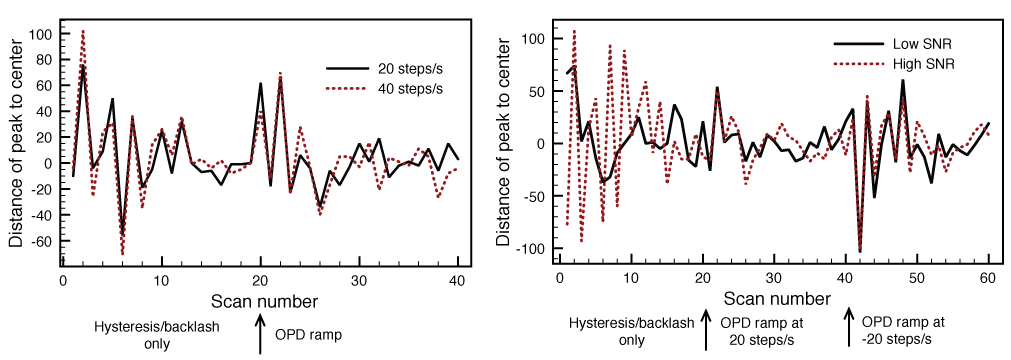
\includegraphics[width=1\textwidth]{Figures/ramps.png}
%{Two snapshots of BETTII's carbon fiber gondola and external optics. To the left, one early design is shown, without most of the holding structures for the optics. To the right, a more recent model is shown, with additional elements to connect the optics and to connect to the balloon train. This structure has exceptional thermal properties, and very high frequency vibration modes.
\caption{Left: Fringe tracking results for one single OPD ramp, showing the distance from the estimated peak from the center of the window in number of steps. The algorithm tries to always keep the peak in the center of the window. The first 20 scans have no perturbation of OPD, and show the algorithm trying to compensate for hysteresis/backlash. Scans 20-40 show the algorithm compensating for an OPD ramp. Right: Fringe tracking results for the two consecutive 20~steps/s OPD ramps of opposite directions, for the two regimes. Note that in this particular run, the initial hysteresis/backlash is not optimally compensated during the first 20 scans in the high-SNR regime, due to initial conditions.}
\label{fig:ramps}
\end{center}
\end{figure}

Algorithm C succeeds at $\sim$~3~Hz tracking of the fringes, only in the high-SNR regime, and provided that we start close enough from the central fringe packet. In the low-SNR regime, dispersed fringes in individual channels have very small SNR and do not permit to identify the phase in each channel. We can only achieve $\sim$~3~Hz because if we operate faster the hysteresis/backlash becomes problematic.



\subsection{Limitations and discussion}
In the current testbed, the reused hardware is our main limitation. The actuators we are using have no absolute encoder, and are turn-screw motors with significant backlash and hysteresis. In addition, synchronization cannot be achieved to a good level, mainly because we are working on a basic Windows machine. The OPD is shown to be stable to the environment when no actuator is in movement (70~nm~rms over 20 seconds, or about 1~step~rms), however, residual noise is injected by vibrational modes caused by the delay lines themselves as they are moved and as they change direction.

Despite these hardware limitations, we successfully achieve robust fringe tracking at low frequency, using broad scans across the fringe packet as shown in the previous section. The actuator backlash and hysteresis, however, prevent us from implementing a fast ABCD algorithm over one wave, since there is too much uncertainty in the step size and shifts in OPD of more than one wave are common. 

Our results are strongly dependent on the size of the fringe packet and on the size of the scan window we choose. Even though our nominal set of parameters achieves sufficient fringe tracking, we do not claim they are optimal. In particular, there is a clear signature of the algorithm that can be seen in Fig. \ref{fig:ramps} Left and Right. Investigating the parameter space to search for optimal values will be done only for flight actuators and sensors in their respective control loops. However, all algorithms developed for the present testbed are generic functions that can easily be transposed to future generations of testbeds and facilitate the search for our optimal set of parameters.

Experimentally, we find that the low-SNR regime is very robust for fringe tracking. This makes us comfortable that we will be able to implement this slow-frequency fringe tracking on BETTII with SNR of about 2.5 on the fringes, as this is enough for the Hilbert algorithm to robustly identify the peak location.

%Hysteresis and backlash are significant and prevent us from implementing a simple ABCD algorithm over just one wave. Thus, our implementation of fringe tracking in preparation for BETTII is still incomplete.



\subsection{The new generation FTU testbed}\label{subsec:newFTU}

In order to enable the ABCD algorithm, and reproduce all operating frequencies used on flight, we are designing an upgraded testbed with candidate actuators and encoders selected for BETTII. This new generation testbed would mimic the AT and FT parts of the flight FTU, and will be controlled by one of BETTII's real-time computer to achieve good synchronization. Although it will have all the same parameters such as the plate scale, Airy disk size, etc., it will work at optical wavelengths for convenience and cost considerations. This new testbed will explore the ABCD algorithm in order to lock on the fringes, and will allow the team to tune almost all algorithms with gains and parameters that are relevant to the flight hardware, while we wait for the dewar to be commissioned. In particular, it will be used to test, align, and calibrate the WDL and the tip/tilt mirrors prior to their integration on the gondola.

\section{Conclusions}

In this paper we describe the design of a NIR fringe tracking unit that will implement angle tracking and fringe tracking for BETTII. The FTU will enable BETTII's science by ensuring optimal beam overlap and OPD knowledge prior the entrance to the dewar. 

The angle tracker will look at the fields from the two arms separately. It will find the guiding star and maintain it at a given position on the detector. The fringe tracker will control the OPD by implementing two motions: the first is an open-loop compensation, fed by the signal from the gyroscopes and the angle tracker. This approximately freezes the fringes. The second motion scans the OPD to find fringes and track any uncorrected OPD. We propose algorithms to achieve $\sim~1$~Hz envelope peak finding and tracking (Hilbert transform), and fast fringe tracking at 25~Hz. One of the two outputs of the fringe tracker is dispersed to provide group delay knowledge.

We built a simple lab setup where we tested different fringe finding and tracking algorithms. This features a traditional Mach-Zehnder interferometer that operates at optical wavelengths. We prove the viability of all algorithms except the ABCD, which requires improved actuators. This testbed is presently being utilized to characterize several candidates for our actuators and sensors at room temperature, before a proper environmental test chamber is built.

A new generation testbed is being designed, that will provide significantly enhanced capabilities, including angle tracking. It will feature improved actuators and absolute encoders, as well as a real-time operating system. This new testbed is designed to allow testing and characterization of BETTII flight tip/tilt mirrors and warm delay line. It will also allow subsystem level testing of the FTU computer and electronics, as well as proper tuning of all relevant algorithms for the different operating modes that BETTII will use in flight.